%
%============= CHAPTER BREAK =================%
%
\chapter{Conclusion}%
%
\vspace*{3mm}
%
\justifying

\noindent{}As the dictum goes: failures are as important, perhaps more important, %
than successes in the progress of Science. %
By way of transparency and recognition of the potential pitfalls of research into the origin points of Greek neologisms, %
here I list words I initially identified as post-Hadrianic neologisms based on TLG queries, %
but later had to discount because of results from queries against databases of Greek papyri and Greek inscriptions. %
If this book is published in a second, corrected edition, %
this section provides a ready-made place to move lemmas from previous chapters %
when and if they are later confirmed as false positives. %

Out of all of the neologism candidates proposed in the first edition, 
undoubtedly some will be disproved as post-Hadrianic. %
How many is difficult to say, but I am cautiously optimistic that the false positive error rate will be 20\% or less. %
If 80\% of these remain and stand the test of time and scrutiny, that should suffice to shift the Overton window %
on the compositional and/or redactional dates of most of the texts in the NT. %
It is also possible that some neologisms currently in the penultimate chapter under %
the NT and early Christian writers will later shift to be classified as non-Christian, post-Hadrianic %
neologisms, if and when they turn up in new editions and additional works by post-Hadrianic Greek authors %
folded into later releases of the TLG, OGA, and GLAUx. %

Finally, it should be said that just because a lemma is demonstrated %
to have emerged before 138 CE does not mean that %
the parallels explored and interdependencies proposed are automatically incorrect. %
For example, even though προεπαγγέλλω is attested before Hadrian, %
the possible influence of Arrian of Nicomedia and his \textit{Alexandri anabasis} %
on the redaction of the canonical Paulines still merits consideration. \clearpage

\section{Flushing False Positives}

\noindent{}\textbf{ἀνακαινόω} / \textit{anakainoō} / “to renew|renovate” (Rom 12:2, 2Cor 4:16, Col 3:10) originally %
fell under the \textit{Acts of Carpus} (\textit{Act.Carp.} 9) in the previous chapter.  %
It was later assessed as a false positive post-Hadrianic neologism %
because the verb clearly registers in an inscription from the famous Dura-Europos %
archaeological site (SEG 37:1442, PH322184, c. 116--117 CE), %
specifically used by the patron (Alexander, son of Epinikos), %
to claim that he had [ἀν]ακαινίσας / “renovated” τὸν ναὸν / “the temple” that his father had built. Even so, %
this finding may point to a late Trajanic or early Hadrianic \textit{terminus post quem} for *2Cor 4:16 and *Col 3:10 (Marcionite and canonical), %
and for canonical Rom 12:2. \\[1mm] %

\noindent{}\textbf{ἀρχισυνάγωγος} / \textit{archisynagōgos} / “synagogue-chief” (Mk 5:22, 35--36, 38; Luke 8:49, 13:14; Acts 13:15, 18:8, 17), %
outside of the NT, is first used in the TLG by Justin Martyr (\textit{Tryph} 137.2), % 
and next by Irenaeus (\textit{AH} 1.1.16). %
Justin intriguingly used the term just before, %
yet syntactically disconnected from, a loose allusion to a “maidenʼs” / κόρης healing. %
By contrast, Irenaeus, Origen, and later readers tend to use it clearly %
in reference to a “synagogue-chiefʼs daughter” / ἀρχισυναγώγου θυγάτηρ, %
perhaps reflecting the later standardization and stabilization of the overlapping canonical Markan-Lukan narrative. %
While these earliest Christian attestations may be valuable %
to show the textual instability of Gospels and Gospel-like traditions %
in the mid-2nd century, they do not actually establish a genuine neologism. %
The term was determined to be a false positive on the basis of the inscription %
JERU0591, Jerusalem, 100BCE--70CE, %
in which the patron uses the lemma twice in quick, genealogical succession: %
ἀ[ρ]χισυνάγωγος, υἱὸς ἀρχισυν[αγώ]γ[ο]υ / %
“synagogue-chief, son of a synagogue-chief”.\endnote{%
The inscription can be confirmed at \url{search.inscriptionsisraelpalestine.org/inscriptions/jeru0591}.} %
This title was commonplace in Jewish epitaphs both within and beyond the city of Rome,\endnote{%
van der Horst 1991:92--93} %
and office-holders could include women.\endnote{\textit{Ibid}., 105--106} \\[1mm] %

\noindent{}\textbf{ἀφεδρών} / \textit{aphedrōn} / “privy” (Mt 15:17, Mk 7:19), based only on TLG results, %
was initially assessed as having its earliest possible non-Christian occurrence %
in the \textit{Partitiones} of [Ps-]Herodian.\endnote{Boissonade 1819:199.} %
This lemma was subsequently determined to be a false positive on the basis of 
OGIS 483 — MDAI(A) 27 (1902) 47,71 — Mys. Pergamon — 199--133 BCE, %
which mentions the management of ἀφεδρώνων / “privies”. \endnote{%
PHI316381, line 233.} \\[1mm] % %

\noindent{}\textbf{θεατρίζω} / \textit{theatrizō} / “to be on stage” (Heb 10:33) %
was initially assessed, based on TLG results alone, %
as a Christian neologism in the neighborhood of ClemAlex (\textit{Strom}. 4.16.101.2). %
It was subsequently shown to be a false positive for a post-Hadrianic neologism %
on the basis of an inscription: Jerash or Gerasa 192, %
in the Syrian Decapolis; %
the inscription dates between 106 and 117 CE.\endnote{JRS 18.1928.153,14 — SEG 7.825.} \\[1mm] % %

\noindent{}\textbf{ἱματίζω} / \textit{himatidzō} / “to clothe” (Mk 5:15, Lk 8:35) %
was initially assessed as a post-Hadrianic neologism tied to one likely authentic %
fragment from Herodianʼs treatise \textit{On Orthography} (Lentz 1867b:500), %
and from another attestation in the long-form \textit{Partitiones} of [Ps-]Herodian (Boissonade 1819:48). %
This was subsequently classified as a false positive %
on the basis of a Greek inscription from Crete dated to the end of the 1st century BCE %
(IG II xi 3 — PH199880 — Diktynnaion). \\[1mm] % %%

\noindent{}\textbf{καταγγελεύς} / \textit{katangeleus} / “declaimer” ostensibly %
has 40 hits in the TLG, but these often conflate the noun καταγγελεύς with %
the verb καταγγέλλω / \textit{katangellō} / “to declare|recite|declaim|denounce”. %
The apparent hit in Epictetus/Arrian is just such a verb, %
thus leaving only Christian attestations to the lemma in the entire TLG! %
It therefore seemed reasonable to conclude that Act 17:18 coined or first popularized the term %
and that Clement of Alexandria (\textit{Strom}. 6.18.166.5) followed suit. %
Despite this initial finding, queries of databases of Greek inscriptions %
turned up a 1st c. BCE hit: IG XII,8 190 — PH79375 — Samothrace.\endnote{%
A second inscription, %
Lesbos — Mytilene — ca. 29 BC — PH74715, %
also seems to use the noun lemma, not the verb.} \\[1mm] % %

\noindent{}\textbf{νιπτήρ} / \textit{niptēr} / “wash-basin” %
was initially thought, based on TLG results, to be a post-Hadrianic neologism %
that appeared first in the \textit{Testament of Abraham} %
and in the long-form \textit{Partitiones} of [Ps-]Herodian. %
But later database searches of Greek inscriptions %
found a clear hit around 200 BCE in ID 372 — PH62846 — TM47818 — Delos.\endnote{%
It also appears in a late, Christian (501--700 CE) Greek papyrus, %
sb 26 16576, on which see \url{papyri.info/ddbdp/sb;26;16576}.} %
The related lemma, ποδανιπτήρ / \textit{podaniptēr} / “foot-wash-basin”, %
appears explicitly in two Attic inscriptions (IG\texitsuperscript{2} 1424a and 1425, or PH3641 and PH3642),
and is also restored for a third (IG\textsuperscript{2} 1427 — PH3644). %
While this finding disqualifies the key lemma %
of the famous Johannine foot-washing scene, %
it may strengthen the case for the influence of Delian Greek inscriptions on the literary artistry %
of the canonical Gospels. \\[1mm] % %

\noindent{}\textbf{ὀνικός} / \textit{onikos} / “of, for, or like a donkey” (Ev 17:2, Mk 9:42, Mt 18:6; % 
 Origen, \textit{Mt.com.} 13.17) originally seemed %
 to be a post-Hadrianic neologism according to TLG results. %
 Later queries of Greek papyri turned up an occurrence ca. 57--56 CE: %
 bgu.8.1782 — TM 4863.\endnote{See \url{papyri.info/ddbdp/bgu;8;1782}.} \\[1mm] % %
 
 \noindent{}\textbf{ὁροθεσία} / \textit{horothesia} / “boundary-fixing” (Acts 17:26) % 
 initially seemed to be a post-Hadrianic neologism, first %
 appearing in non-Christian writings in the TLG in the late 2nd or early 3rd century. %
 But the lemma is attested in a Greek inscription at Delphi (FD III 4:42) %
 at the end of the 2nd century BCE. %
 There are, however, several Greek inscriptions in Greece and Macedonia %
 spanning from late in Trajanʼs reign to that of Hadrian, %
 which may suggest an increased popularity around that time. \\[1mm] % %

 \noindent{}\textbf{πληροφορία} / \textit{plērophoria} / “full-assurance|full-satisfaction” (Col 2:2, 1Thes 1:5, Heb 6:11, 10:22; %
 Ps-Clem, \textit{1Cor} 42.3, Ign13 \textit{Magn.} 3.11; Irenaeus, \textit{Fr.deperd.} 27) %
 initially seemed to be a genuine Christian neologism. %
 The lemma, though supplied/reconstructed, %
 was later confirmed as a highly likely reading in P. Giss. 1 87, lines 25--26, which dates ca. 113--120 CE.\endnote{% %
 TM 19474 — \url{papyri.info/ddbdp/p.giss;1;87}.} 
 %
 The verbal lemma πληροφορέω / \textit{plērophoreō} / “to satisfy fully” %
 was apparently attested as far back as the 5th or 4th century BCE in Ctesias.\endnote{%
 \textit{Fragmenta}, Jacoby 3c,688,F, frag. 14, line 75. %
 It also made a pre-1st century CE appearance in LXX Ecclesiastes 8:11.}
 πληρ- / \textit{plēr}- prefixes are largely absent from the Marcionite texts, but prevalent in the canonical texts, %
 on which see the independent, mutually confirmatory findings in IDD and \textit{CPCNT}. %
 Even so, the canonical redactors here apparently did not invent a new term so much as %
 borrow one known and used in Roman Egypt, in the well-known archive of the governor Apollonius, %
 with a late Trajanic or early Hadrianic date. %
 The novelty of the canonical Christian usage was perhaps in the %
 appropriation of a clearly financial term for religious and philosophical discourse. \\[1mm] % %

\noindent{}\textbf{πολιτάρχης} / \textit{politarchês} / “civic magistrate” (Acts 17:6, 8; 4th--5th c. varia) %
seemed, on initial review of TLG results, to be a genuine Christian neologism. %
It appeared twice in Acts and subsequently in various 4th and/or 5th century compositions.\endnote{%
The first of these is difficult to determine without further research: \textit{Acts of Phillip} 46--50; Symeon the Mesopotamian, \textit{hom}. 26.1.9; %
twice in the \textit{Epistula canonica} associated with Peter I of Alexandria, %
and 12 times (!) in the \textit{Acts of John by Prochorus}, %
which Spittler (2023:272--273) dates between the early 5th and early 7th century.} %
πολίταρχος / \textit{politarchos}, the second declension noun, had appeared in the 4th c. BCE Aeneas, %
\textit{Poliorcetica} 26.12.\endnote{%
But not subsequently in the TLG until 9th century CE and later!} %
However, a search of digitized Greek papyri turned up various pre-1st century CE examples %
of the first declension lemma.\endnote{%
E.g.: EKM 1 1 — SEG 27.261 — SEG 43.381 — PH149475; Mel. 11 44,A2 — SEG 42.558 — PH152405.} \clearpage % %

\noindent{}\textbf{ποταμοφόρητος} / \textit{potamophorētos} / “carried off by a river”, %
according to TLG results, appears first in the Greek magical compilation known %
as the \textit{Cyranides} 1.20 (late 4th or 5th century CE, though possibly reliant on late 2nd century sources), %
as well as in the NT Revelation (12:15). %
LSJ cites a couple of papyri, including a Greek magical papyrus (PMag.Par.1.876 — PGM IV.876, early 4th century, %
but again possibly reliant on 2nd century material), %
as well as PStrassb.5.10 (3rd c. CE). %
But another Greek papyrus (p.hib. 2 265 — TM 8292), dated between 204 and 203 BCE, %
already contained the lemma. \\[1mm]

\noindent{}\textbf{πρόκριμα} / \textit{prokrima} / “prejudgement”, %
based only on TLG results, %
appears first in 1Tim 5:21, and next in ClemAlex, \textit{Strom}. 1.1.4.4. %
While the term only seems to appear in Greek papyri during the 4th century (8 hits), %
it is attested in an inscription from 42--30 BCE (IGSyr 3,1 718, PH242797), %
as well as an inscription from 44 CE in Ephesus (Ephesos 227 — Ephesos 228; PH247934 — PH247935). \\[1mm]

\noindent{}\textbf{προεπαγγέλλω} / \textit{proepangellō} / “to pre-promise|pre-announce” %
appears some 185 times in total in the TLG, %
but did not turn up in initial searches of major databases of Greek papyri or inscriptions. %
In response to my first edition, %
Carrier ran searches of the Packard database (which I did consult, %
but not for this termʼs aorist forms, as I should have), %
and found two examples, though incorrectly listing them as four different artifacts, %
“an 84 B.C. Priene inscription, and in an inscription from the 2nd/1st BC, %
and another, and another of the 1st century BC”.\endnote{Carrier 2026.} %
But two of the four are duplicates. %
προεπ̣ηγγελμέν[α] / \textit{proepēngelmen[a]} appears in Priene 33 %
— IK Priene 69 — Ionia — after 84 BC — IvPriene (1906) 113. %
προεπηγγείλατο / \textit{proepēngeilato} appears twice %
(once with a lacuna restored as [πηγ] / [\textit{pēn}]) %
in Priene 209 — IK Priene 184 — Ionia — 2nd/1st BCE — SEG 31.983. %

Its first hit in a non-Christian prose text is subsequently found within the \textit{Alexandri anabasis} of Arrian. %
Scholars debate the date of this composition, %
not least because of the ambiguity of Arrianʼs “second preface” to the work. %
Syme favored an early or late Antonine date, after Arrianʼs time as %
legate and governor of Cappadocia.\endnote{%
Syme 1982:209.} %
Stadtler situated the \textit{Anabasis} as either late Hadrianic (Cappadocian) or early post-Hadrianic (Athenian).\endnote{Stadtler 1980.} %
Moles was more confident about its post-Hadrianic composition in Athens.\endnote{%
Moles 1986:168 points to an identical phrase in the \textit{Cynegeticus} / \textit{On Hunting-Dogs}, %
which was composed after 140 CE in Athens, as well as to the “tremendous self-confidence” %
and sense of literary legacy conveyed in the preface.} 
Other scholars have argued for an early Hadrianic date,\endnote{%
Leon 2021, esp. the appendix, “The Date of the Anabasis”.} %
or maintained that the date puzzle is unsolvable.\endnote{%
Bosworth 1982.} %
Alexander the Great was conspicuously missing from several of Arrianʼs earlier writings, %
and it may have been his military leadership in Cappadocia to repel the Alani and subsequent composition of the \textit{Tactica} late %
in his governorship that inspired him to take a keen interest in Alexanderʼs military tactics and career. %

The relevant lemma appears amidst Alexanderʼs exploits \textit{en route} to India, %
specifically in Gadrosia, %
what is modern day Balochistan. %

\vspace*{2mm} 
 \begin{quote}Ὡς δὲ ἀφίκετο ἐς τῶν Γαδρωσίων τὰ βασίλεια,
 ἀναπαύει ἐνταῦθα τὴν στρατιάν. %
 καὶ Ἀπολλοφάνην μὲν παύει τῆς σατραπείας, %
 ὅτι οὐδενὸς ἔγνω ἐπιμεληθέντα τῶν \textbf{προεπηγγελμένων}, %
 Θόαντα δὲ σατραπεύειν τῶν ταύτῃ ἔταξε· %
 τούτου δὲ νόσῳ τελευτήσαντος Σιβύρτιος τὴν σατραπείαν ἐκδέχεται· (\textit{Alex.anab.} 6.27.1) \\[1mm] %
 But as he arrived at the royal courts of the Gadrosians, %
 he was resting the army there. %
 And he fired Apollophanes from the satrapy, %
 because he knew nothing of managerial duties of those \textbf{pre-promised}. %
 He stationed Thoas to be satrap of things there. %
 But when he perished by sickness, Sibyrtios received the satrapy. %
 \end{quote} % 
 \clearpage

\noindent{}In later non-Christian writings, %
the lemma appears once in a word list of Julius Pollux (\textit{Onomast}. 5.105), %
and became more popular with Cassius Dio, who used it no less than seven times.\endnote{%
\textit{H.R.} 36.39.1, 38.13.5, 39.31.1, %
40.32.3, 42.32.3, 46.40.2, 59.21.2.} %

In the NT, the lemma appears twice, both in canonical Pauline verses %
likely missing from Marcionʼs \textit{Apostolos} (2Cor 9:5, Rom 1:2): %

\vspace*{2mm} 
 \begin{quote}\textls[-15]{ἀναγκαῖον οὖν ἡγησάμην παρακαλέσαι τοὺς ἀδελφοὺς %
  ἵνα προέλθωσιν εἰς ὑμᾶς καὶ προκαταρτίσωσιν τὴν \textbf{προεπηγγελμένην} εὐλογίαν ὑμῶν, %
 ταύτην ἑτοίμην εἶναι οὕτως ὡς εὐλογίαν καὶ μὴ ὡς πλεονεξίαν.} \\[1mm] %
 So I considered it necessary to exhort the brothers, %
 so that they might pre-arrive to you and pre-furnish the \textbf{pre-promised} blessing of yours, %
 this prepared so as to be a blessing and not as greediness.\end{quote} % 
 \vspace*{1mm}

 \begin{quote}Παῦλος δοῦλος Χριστοῦ Ἰησοῦ, κλητὸς ἀπόστολος, ἀφωρισμένος εἰς εὐαγγέλιον θεοῦ, %
 ² ὃ \textbf{προεπηγγείλατο} διὰ τῶν προφητῶν αὐτοῦ ἐν γραφαῖς ἁγίαις (Rom 1:1--2) \\[1mm] %
 Paul, a slave of Christ Jesus, called apostle, %
 having been separated for the evangelion of God, %
 ² which was \textbf{pre-promised} through his prophets in holy scriptures.\end{quote} % 
 \vspace*{2mm} %

 With Arrianʼs usage as background, %
 canonical Paul enacts an antithesis to Apollophanes. %
 Whereas Alexander ended the political career of the former, %
 Paul himself, and those under his charge, are fully aware and totally devoted to their %
 responsibilities to “what was pre-promised”. %
 Both canonical NT usages match Arrianʼs as passive forms made substantive by the preceding word. %
 Whereas the preceding pronoun and regular verb in Rom 1:2 are somewhat distinctive, %
 2Cor has a closer match: a definite article precedes the participial form of the lemma. %
 The literary juxtaposition of Paul with Apollophanes is also befitting %
 as a form of literary imitation and rivalry of a notable Apollo-theophore.\endnote{%
 For an expansion of the thesis of Paul as Apollo-theophore, %
 contrasted with the villainous Apollonius of 4 Maccabees, see Bilby 2026, chp. 8.} %

\noindent{}\textbf{πρωτοκλισία} / \textit{prōtoklisia} / “first-seat” %
first seemed to be an NT neologism: *Ev 11:43, Mt 23:6, Mk 12:39, Lk 14:7--8, 20:46, %
followed by ClemAlex, \textit{Paed}. 2.1.4.5. %
A search of Greek inscriptions, though, returned ID 1520 — PH63945 — AGRW 224 — AGRW 1576 — Delos — post 153/152 BCE. %
A Greek papyrus has a supplied instance: sb 6 8993 — p.harr.1.61 — TM 5720 — possibly from Oxyrynchus — 176--175 BCE. \\[1mm]

\noindent{}\textbf{τεκνογονέω} / \textit{teknogoneô} / “to bear children” (1Tim 5:14), %
has 109 TLG hits in total, no Greek papyri or inscriptions listed as such in LSJ, %
and my searches of major databases also turned up empty. %
It thus first seemed to me a non-Christian, post-Hadrianic neologism %
found in an extant fragment of \textit{Basilica}, %
book one of Appianʼs \textit{Historia Romana}. %

\vspace*{3mm}
 \begin{quote}Πρόκας καὶ τρισκαιδέκατον Νεμέτωρ καὶ Ἀμούλιος. %
 τούτων ὁ πατὴρ Νεμέτορι ὡς πρεσβυτέρῳ τὴν ἀρχὴν κατέλιπεν· %
 Ἀμούλιος δὲ ὁ ἀδελφὸς παρωσάμενος αὐτὸν ἐβασίλευσεν· %
 ὑποπτεύων δὲ τὴν τίσιν Ἔγεστον μὲν τὸν
 υἱὸν τοῦ ἀπωσμένου ἀναιρεῖ ἐν κυνηγεσίῳ, %
 τὴν δὲ ἀδελφὴν αὐτοῦ δεδιὼς παῖδα εἰ \textbf{τεκνογονήσοι}, ἱέρειαν καθίστησιν. %
 (\textit{H.R. Basilica}, fr. 1a.6)\endnote{%
 Viereck \& Roos 1962:16.} \\[1mm] %
 Procas and Numitor the 13th and Amulius. %
 Their father left the rule to Numitor as the eldest. %
 But Amulius, his brother, reigned after pushing him aside. %
 Then suspecting payback, he took out Aegestus, %
 the son of the exiled [ruler], on a dog-hunt. %
 Dreading that his daughter \textbf{might child-bear} a child, %
 he ordained her a priestess. \end{quote} % 
 \vspace*{2mm}

LSJ also cited an excerpt from the \textit{Anthologia Graeca}, %
specifically Epigram 9.22 attributed to “(Phil.)”, %
a citation that I initially overlooked. %
Subsequent research confirmed its attribution to the mid-1st century CE epigram compiler, %
Philip of Thessalonica.\endnote{%
\url{anthologiagraeca.org/passages/urn:cts:greekLit:tlg7000.tlg001.ag:9.22}. %
The excellent Anthologia Graeca website has a cropped manuscript image preview and %
link to Cod. Palatinus 23, p. 361, %
along with a transcription and several translations. %
It confirms this lemma in the TLG text from Beckby 1968, vol. 3.} %
As Plastira-Valkanou notes, %
Philip of Thessalonica compiled his \textit{Garland} of epigrams %
in “emulation of Meleager” and has proven to be an “underestimated”, “creative poet”. %
Philip was particularly known for coining new words, %
“mostly compound nouns, adjectives, and verbs”.\endnote{%
Plastira-Valkanou 2023.} %
And while “some of these” may have originated in earlier texts, %
“100 of Philip’s neologisms do not reappear in later authors”.\endnote{\textit{Ibid}.} %

τεκνογονέω / \textit{teknogoneô} may well be one of these neologisms, %
and Appian may well have picked up this neologism from Philip or one of his subsequent imitators. %
This exploration invalidated the lemma as post-Hadrianic. %
However, the question remains, where did canonical 1Tim pick up the rare/new lemma? %
Was it directly from Philipʼs epigrams? From one of his unknown imitators? %
Or was it still by way of Appianʼs famous and enormously popular \textit{Historia Romana}? %
My wager is on the latter, %
both for the NT usage and for its occurrence in the famous \textit{Epistle of Diognetus}. %
I reproduce the quotation of the Pastoral epistle to invite your pondering of the question. %

\vspace*{2mm} 
 \begin{quote}βούλομαι οὖν νεωτέρας γαμεῖν, τεκνογονεῖν,
 οἰκοδεσποτεῖν, μηδεμίαν ἀφορμὴν διδόναι τῷ ἀντικειμένῳ
 λοιδορίας χάριν· \\[1mm] %
 Therefore, I counsel younger women to marry, to bear children, %
 to house-master, giving no occasion at all to the opposer %
 as a cause of slander. \end{quote} %
 \vfill{}

\noindent{}\textbf{φρεναπάτης} / \textit{phrenapatēs} / “soul-deceiver”, %
an NT \textit{hapax}, first seemed a post-Hadrianic %
neologism. The quotation of Tit 1:10 follows: %%
\vspace*{3mm}

\begin{quote}Εἰσὶν γὰρ πολλοὶ [καὶ] ἀνυπότακτοι, ματαιολόγοι καὶ \textbf{φρεναπάται}, %
 μάλιστα οἱ ἐκ τῆς περιτομῆς / For many are unrestrained, empty-talkers and \textbf{soul-deceivers}, %
 especially those of the circumcision \end{quote} \clearpage

\noindent{}It also appears in a fragment of Herodianʼs authentic \textit{Peri figura},\endnote{%
See Dickey 2014:340 on the authenticity of the first Περὶ σχημάτων / \textit{Peri figura} / \textit{On Compounding}, %
which is preserved only in fragments and should not be confused with the longer form %
work of the same name, but which is about rhetorical figures.} %
whose quotation follows (\textit{fig}. \textit{GG} 3.2:848): % 

\vspace*{3mm}
 \begin{quote}καὶ εἰ μὲν ἡ ἐπιφερομένη λέξις ἄρχεται ἀπὸ συμφώνου, %
 ἀποβάλλει ἡ γενικὴ τὸ ς οἷον φρήν φρενός φρενοβλαβής %
 ... ἐὰν δὲ ἀπὸ φωνήεντος ἄρχηται, %
 ἀποβάλλεται καὶ τὸ ο καὶ τὸ ς οἷον φρήν φρενός \textbf{φρεναπάτης} \\[1mm] %
 And whenever the compounded word begins with a consonant, %
 the genitive casts off the final \textit{sigma}, such as: %
 mind (\textit{phrēn}), of mind (\textit{phrenos}), deranged (\textit{phrenoblabēs}) ... %
 but if it should begin with a vowel, %
 both the \textit{omicron} and the \textit{sigma} is cast off, %
 such as: mind (\textit{phrēn}), of mind (\textit{phrenos}), \textbf{soul-deceiver} (\textit{\textbf{phrenapatēs}})\end{quote} % 
\vspace*{3mm}

LSJ cited the 6th century CE PLond.5.1677.22 for the lemma. %
The next results in the TLG were Origenʼs responsive comments in \textit{Cels}. 3.48, %
where they perhaps allude to Tit 1:10. %
It also appears in Ign13, \textit{Trall}. 6.2, which quotes Tit 1:10. %
The LSJ also cited Lyr.Alex.Adesp.1.18, which I initially dismissed, %
since it was not listed near the top of the date-sorted TLG hits. %
(I honestly have no idea why this happened. Try the lemma search yourself and see what you find! %
Could it perhaps be a software bug or perchance an incorrect bit of metadata?) %
I supposed that its anonymous authorship reflected a situation comparable %
to the various strata of late love poetry found in the \textit{Anacreonta}. %

Further research led down quite an enjoyable, poetic rabbit-hole. 
In Powellʼs edition\endnote{Powell 1925:177--178.} %
and in the TLG, Lyr.Alex.Adesp. 1.18 was eventually found and confirmed %
as an anonymous, fragmentary Greek lyrical song with the heading, %
Παρακλαυσίθυρον / \textit{Paraklausithyron} / “Standing outside Door”, %
a motif in Latin known as \textit{Exclusus amator} / “the Shut-out Lover”, %
one quite developed in Ovidʼs Latin poetry.\endnote{Copley 1956.} % 
According to Copley, Plutarch was the first to use this specific Greek word as a classification %
for a type of song that in classical sources was simply called κῶμος / \textit{kōmos} / “revel”, %
i.e., a song sang by intoxicated men at the conclusion of or subsequent to a symposium, %
often in front of the homes and doors of available women.\endnote{%
On Plutarchʼs attestation, see Copley 1942:97, citing \textit{Amat}. 8.753B.} %
This to me suggested a 2nd century CE date at the earliest for this particular fragment, %
and its use of the rare and apparently new lemma φρεναπάτης / \textit{phrenapatēs}. %

However, further research confirmed that this song, including its lemma φρεναπάτης / \textit{phrenapatēs}, %
are both explicitly attested by a 2nd century BCE papyrus. %
This papyrus is known alternatively as the \textit{Fragmentum Grenfellianum}, %
after its discoverer who first published the Oxyrynchus papyri, %
or as P. Dryton 50, after the name of the Roman Egyptian officer of the 2nd century BCE %
who transcribed these lines.\endnote{Battezzato 2009:404.} %
All of this confirmed the lemma was a false-positive post-Hadrianic neologism. %
This research adventure may also be something of a cautionary tale, %
a summons to humility instead of hubris about all the knowledge inaccessible to the composer of this volume, %
and a reminder that this scientific quest (or is it a musical apocalypse?), %
even if it has stumbled upon some forty-odd beacons of authentic light from our human past, %
may be little more than the rantings of a blind fool fumbling around in the dark. \clearpage

\section{Challenged \& Uncertain Neologisms}

\noindent{}Some neologism candidates detailed in the first edition have met with criticism, %
particularly the introductory example, %
which was the inspiration for the line of research into potential post-Hadrianic neologisms, %
not necessarily its strongest example. %
In this supplemental section new to version 1.2, %
I recount the basic case presented in the first edition for this opening neologism candidate, %
note some of the criticisms made, %
and respond to explain why I am not yet convinced it %
can yet reasonably be dismissed as a false positive post-Hadrianic neologism that first originated, %
or was at least first popularized, outside of the canonical Acts of the Apostles. \\[1mm]

\noindent{}\textbf{κατείδωλος} / \textit{kateidōlos} / “full of idols” on preliminary inspection %
seemed to be a term that was coined or first popularized by Polyaenus. %
The \textit{Oxford Classical Dictionary} says Polyaenus was a “Macedonian rhetorician” %
who composed the \textit{Strategemata} in the 160s CE, dedicating it personally to the emperors %
Marcus Aurelius and Lucius Verus. %
This page of TLG results shows the initial evidence evaluated: %

\vfill{}
\begin{figure}[h!]
    \centering
    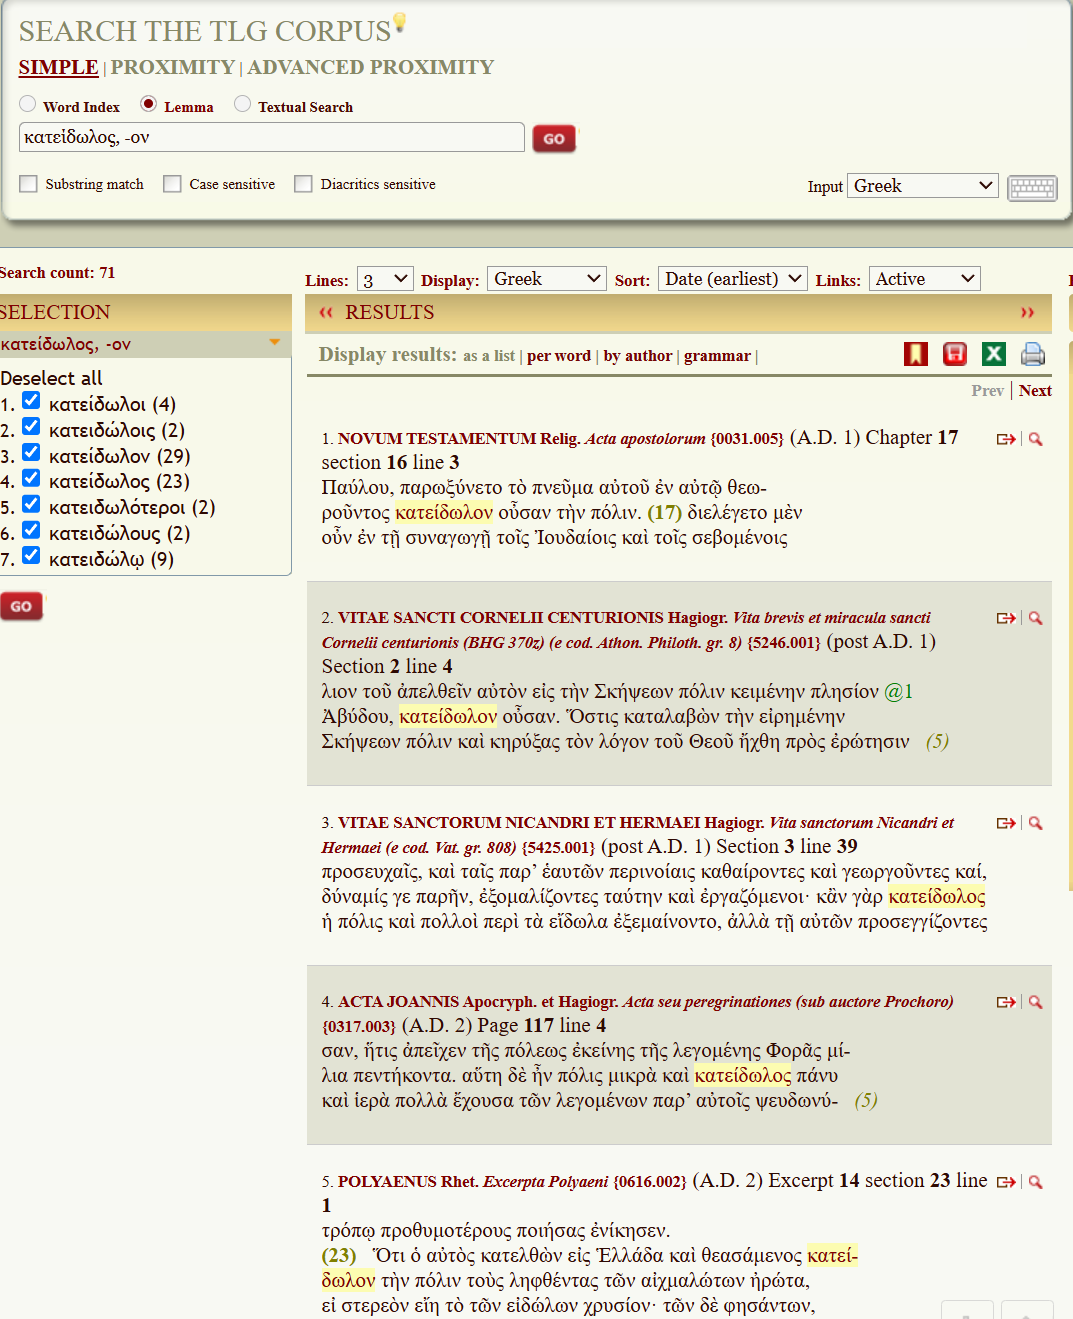
\includegraphics[height=0.85\textheight, width=.95\textwidth]{images/ch24_kateidwlos_TLG.png}
    \caption{TLG Search Results: κατείδωλος}
    \label{fig:kateidolos}
\end{figure}
\clearpage

Hits 2--4 in the TLG results all appear in lives/acts of %
Christian saints (Cornelius Centurion, Nicander and Hermaeus, and John by Prochorus). %
Though the TLG metadata assigns all of these to the 1st century CE, %
this dating is unsupported by any evidence, not maintained by any current scholar, and almost certainly incorrect. The excerpt from Polyaenus (hit 5) runs as follows: 

\vspace*{3mm} 
 \begin{quote}Ὅτι ὁ αὐτὸς κατελθὼν εἰς Ἑλλάδα καὶ θεασάμενος %
    \textbf{κατείδωλον} τὴν πόλιν τοὺς ληφθέντας τῶν αἰχμαλώτων ἠρώτα, %
    εἰ στερεὸν εἴη τὸ τῶν εἰδώλων χρυσίον· (\textit{Excerpta} 14)\endnote{%
    Woelfflin \& Melber 1970:449.} \\[1mm]
 He himself, after descending into Greece and observing the city was \textbf{full of idols}, %
 asked those of the captives being held, if the gold of the idols was solid.\end{quote} %
\vspace*{3mm} %

In a public review of the introduction and first chapter of the first edition of this book, %
Carrier helpfully pointed out that the key elements of this excerpt that overlap with Acts %
are largely missing from the better attested %
and more extensive text of the \textit{Stategemata} at 7.35.2.\endnote{%
Carrier 2026.} %
Carrier rightly pointed to the cautions and observations by Woelfflin and Melber %
about the \textit{Excerpta Polyaeni} being a later abridgement by an epitomizer. %
He also aptly corrected my mistaken assumption that the excerpt attributed to Polyaenus %
was referring to Athens, when in light of its proper and fuller context in the main text of %
the \textit{Strategemata} that Woelfflin and Melber cross-index, %
this episode was clearly situated in Delphi. %
I also mistakenly associated Brennus, the 3rd century BCE invader of Greece, %
with a different Brennus who sacked Rome in the 4th century BCE. %
On all of these points I stand corrected. %

Amidst these criticisms, %
Carrier still admitted that the episode in Acts evidences numerous, dense, and sequential parallels with the excerpt %
that cannot be reasonably explained as mere coincidence: % 

\vspace*{3mm} 
 \begin{quote}Ἐν δὲ ταῖς Ἀθήναις ἐκδεχομένου αὐτοὺς τοῦ Παύλου παρωξύνετο %
    τὸ πνεῦμα αὐτοῦ ἐν αὐτῷ θεωροῦντος \textbf{κατείδωλον} οὖσαν τὴν πόλιν. \\[1mm]
\textls[-10]{Now when Paul was received by them in Athens, %
 the spirit of his in him was provoked when he was spectating the city being \textbf{full of idols}.} %
 \end{quote} % 
 \vspace*{3mm}

A close comparison of the two texts shows a similarity beyond one extremely rare word. %
Both passages associate the term with a “city”, and in particular a major, opulent Greek religious center. %
Even more strikingly, the word form (accusative singular), syntactical parent (πόλιν / “city”), %
and trailing neighbors are identical, except for one intervening word (οὖσαν / “being”): %
“full of idols […] the city” / κατείδωλον […] τὴν πόλιν.\endnote{%
The Democritus example and similar Attic examples adduced by Carrier, which clearly use a preposition (κατ’) + genitive plural noun (εἰδώλων) %
+ accusative noun (ἐμπτώσεις | ἐνστάσεις) construction, %
are too dissimilar to the adjectival lemma in morphology and syntax %
to be considered a solid match or establish a pre-Hadrianic attestation %
according to scholarly standards and rules of lexicography. %
Epicurean Attic philosophy about the nature and travel of light and perception (images as effluences that enter the eye) %
is also not a close thematic match to the focus on travel, opulence, religious statues, and potential plunder uniquely shared between Polyaenus and Acts. %
While it is technically true that the \textit{omega} did not exist in many of the earliest Greek scripts, %
that \textit{omicron} could be understood as conveying a long “o” sound, %
that \textit{omicron} and \textit{omega} were sometimes (though not typically) confused by scribes and epigraphers, %
and that \textit{scripta continua} could in these specific conditions look identical to our lemma, %
Carrierʼs line of criticism in this regard is too clever by half, to the point of bordering on the pretentiously absurd. %
The prefix of our adjectival lemma carries an implicit accusative sense (idols everywhere, all the way down!), modifying the word “city”, %
not a genitive sense, as in the philosophical commonplace of “impacts from images”.} %
Both passages use the lemma κατείδωλος to describe the main character as a figure from the past %
who observes the city he visits, apparently for the first time. %
Though the verbs of seeing differ, both happen to be participles with identical opening and closing letters %
(cp. θεασάμενος and θεωροῦντος). %

While I initially viewed Acts as depending on the \textit{Strategemata} of Polyaenus, %
that now needs to be qualified as uncertain, tied up in textual evolutions far more complex than I first appreciated. %
Carrier speculates when claiming that the \textit{Excerpta Polyaeni} comprise an epitome by %
“an unknown Medieval Christian redactor (maybe of the 6th century).” %
He continues on firmer ground: that the \textit{Excerpta} are preserved %
“via manuscripts of the 10th and 11th centuries (see Melber \& Woelfflin, \textit{Polyaeni strategematon libri} viii, xix, 346, 449).” %
In context, Woelfflin and Melber discuss the \textit{Strategems} of Emperor Leo I, %
but they do not claim that their critical text of the %
\textit{Excerpta Polyaeni} itself reflects a 6th century Christian composition. %
It may be that Carrier was confused by their reference to the \textit{Strategems} of Emperor Leo I (457--474 CE). %
But Leoʼs \textit{Strategems} are not identical to the \textit{Excerpta Polyaeni}; %
they instead made use of the earlier \textit{Excerpta} %
and did not draw directly on the \textit{Strategemata} of Polyaenus. %
This earlier epitome is entitled the %
ὑποθέσεις τῶν ἐκ τῶν στρατηγικῶν πράξεων / %
\textit{Summaries of Matters from Military Deeds}.\endnote{Woelfflin \& Melber 1970:xxi.} %
As Dain has covered more extensively, these \textit{Hypotheseis} (i.e., our \textit{Excerpta}) was the earliest among, %
and basis for, no fewer than four other thematically-organized Byzantine epitomes %
of Polyaenusʼ massive and disorganized \textit{Strategemata}.\endnote{%
Dain 1931.} 

A Christian redaction would have lent support to Carrierʼs counterclaim of %
reverse dependence, i.e., the \textit{Excerpta} depend on Acts. %
But further research is needed to explore the date of \textit{Hypotheseis} %
and whether it contains any other confirmatory traces of Christian editing or scripturalizing %
(i.e., inserting cross-references or allusions to Christian scriptures). %
The study of Polyaenus and of compendia of military strategies are scholarly specializations in their own right, %
and it may be wisest to consult more seasoned experts on these matters. %
